
\chapter{ Format all the things }

In a Nrwl setting, we have a format npm script that is available to us by default.
It is called:

\begin{verbatim}
  nx format write
\end{verbatim}

This will call, a .prettier file that has been created by the nx workspace
command. Prettier is similar to to the CLI to the extent that there is a lot
that is happening behind the scenes. In short, it will automatically format files
for you, to it's liking. It's like a pro-active linter, that will format code
for you.

Two architectural talking points, with regards to prettier:
\begin{enumerate}
  \item You will have to format your tslint, so that it does not compete with prettier.
  \item You are going to want to hook up prettier with your IDE, so prettier
  can go to work without having to run it in your terminal.
\end{enumerate}

Note: We are going to have to create a way that we can update the prettier file
automatically.

\section{ How to add prettier to Webstorm }
As we mentioned in a previous chapter, Webstorm is our IDE of choice. VIM users
and Atom users, I completely respect your decision, and feel free to code in
that capacity. However, my experience working with large teams, is  that Webstorm
has a lot to offer outside of the box. For the non power user, it will offer
all of those benefits. Ok, great, the following is how to add prettier to Webstorm
with a screenshot!

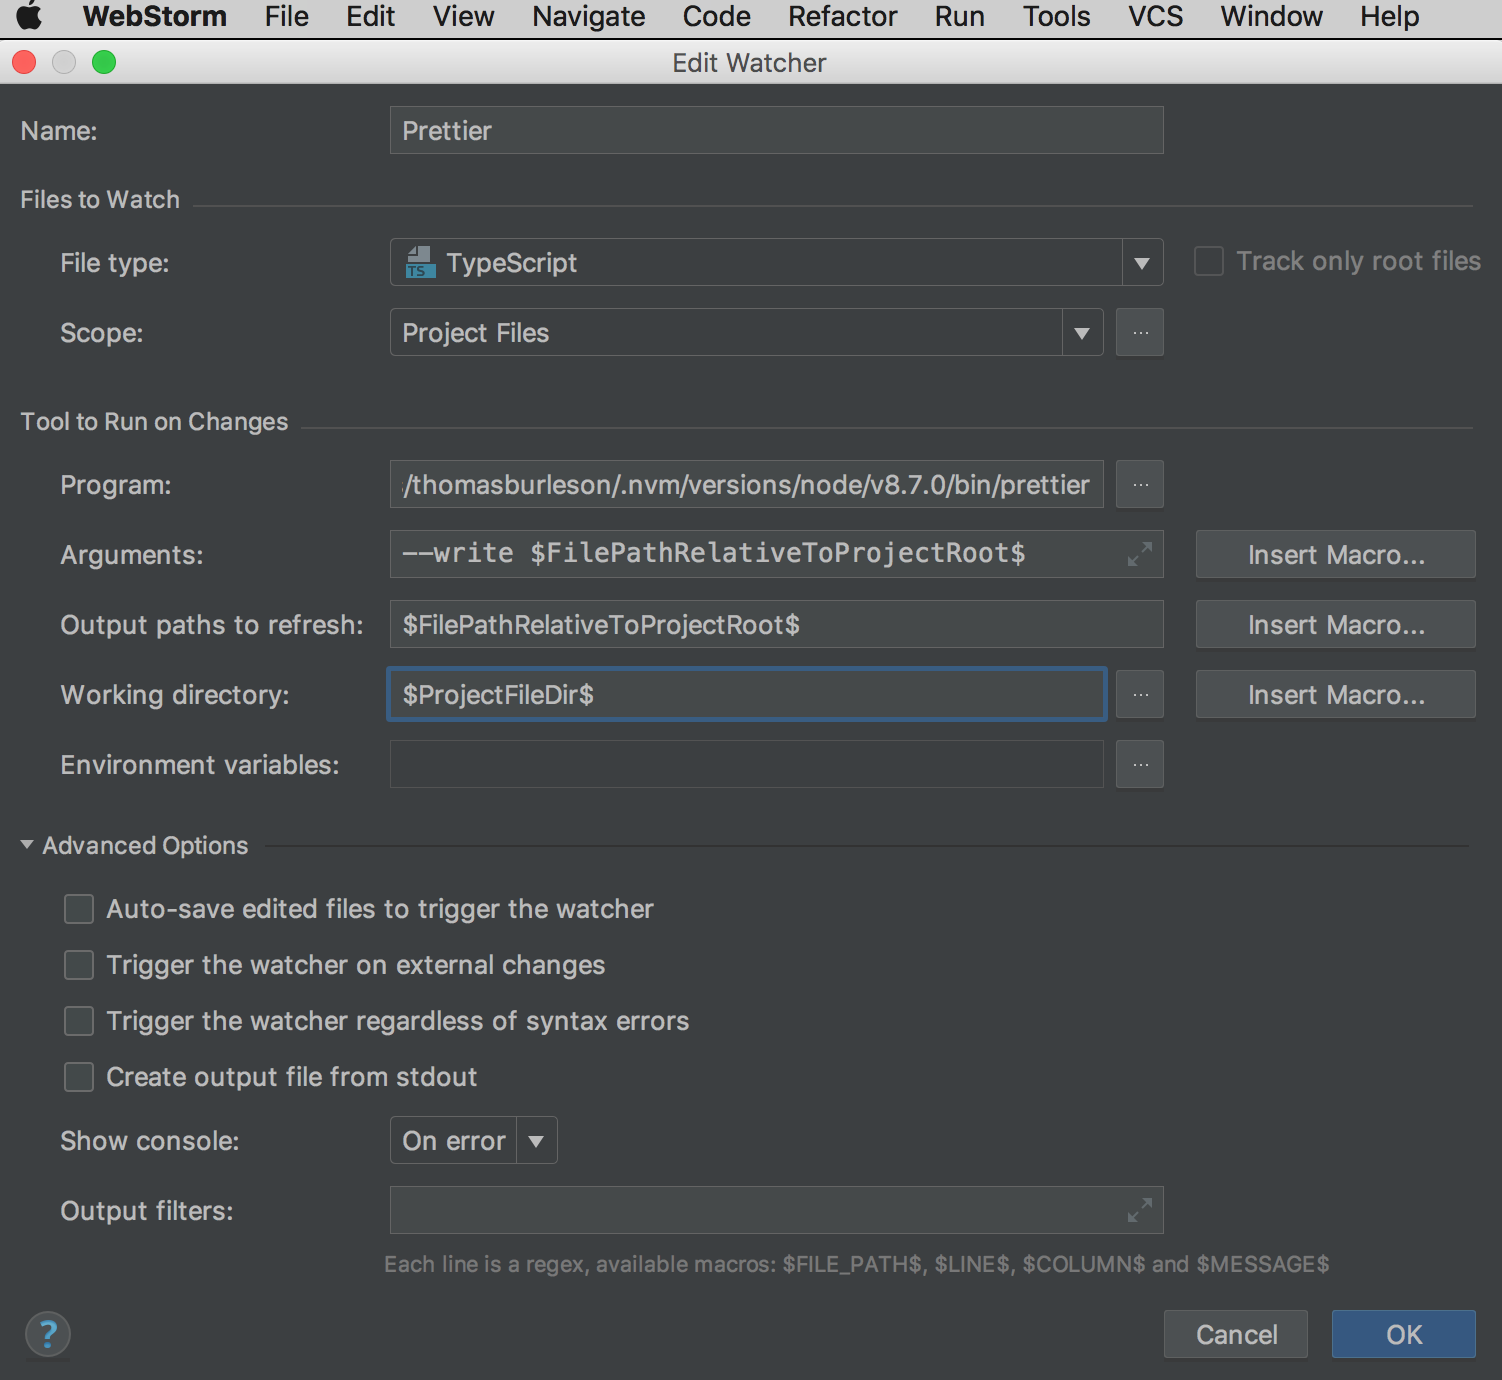
\includegraphics[scale=0.5]{linting/format-all-the-things/prettier-file-watcher-webstorm}
